\section{Systematics}

The analysis performances both the statistical fit to MD distribution to extract the EW-ZZjj contributions
and the cross section measurements in fiducial volume.
Therefore, theoretical and experimental uncertainties may affect the predictions background yields and shapes, 
correction factors from detector-level to particle-level measurement, as well as the $ZZjj$ MD shapes and so on.
Moreover, the statistical uncertainties of simulated samples are also taken into account.
And due to the extramely low cross section of \llll channel, the analysis is still data statistic dominanted.
This section will described the measurement of both theoretical and experimental systematics for $ZZjj$ productions.
The systematics for fake backgrounds have been elaborated in section~\ref{sec:fake_syst}.

\subsection{Theoretical systematics}

The theoretical systematics on EW- and QCD-ZZjj processes include the uncertainties from PDF, QCD scale, $\alpha_{S}$ and parton showering variations.
The PDF uncertainty is estimated from envelop of NNPDF internal variations and the difference between nominal and alternative PDF sets, following the PDF4LHC as introduced in section~\ref{hadroniccollision}.
The QCD scale uncertainty is estimated by varying the nominal renormalisation scale ($\mu_{R}$) and factorisation scale ($\mu_{F}$) by a factor of 0.5 or 2.0.
There are seven different configurations being considered, where the maximum of variations is choosen as final uncertainty.
The parton showering uncertainty is estimated by comparing events with different parton showering setting between the nominal \textsc{Pythia8} and the alternative \textsc{Herwig7}\cite{Bellm:2015jjp, Bahr:2008pv} algorithm.
The $\alpha_{S}$ uncertainty is estimated by varying the value of $\alpha_{S}$ within \pm 0.001.
Details of those variation components are summarized in table~\ref{tab:syst_theo_uncer}.
\begin{table}[!htb]
\small
\begin{center}
\begin{tabular}{p{5cm}p{5cm}p{5cm}} 
\hline\hline
Process     & EW-ZZjj   & QCD-ZZjj \\
\hline
PDFs        & NNPDF30lo (nominal), CT14lo & NNPDF30nnlo (nominal), MMHT2014nnlo68cl, CT14nnlo \\
\hline
$\alpha_{S}$ & 0.118 & 0.117, 0.118 (nominal), 0.119 \\
\hline
QCD scale ([$\mu_{R}$, $\mu_{F}$]) & [0.5,0.5], [0.5,1], [1,0.5], [1,1], [1,2], [2,1], [2,2] & [0.5,0.5], [0.5,1], [1,0.5], [1,1], [1,2], [2,1], [2,2] \\
\hline 
Parton showering algorithm & Pythia8, Herwig7 & - \\
\hline\hline
\end{tabular}
\caption{
Summary of different variations for EW- and QCD-ZZjj theoretical uncertainties measurement.
}
\label{tab:syst_theo_uncer}
\end{center}
\end{table}
Due to the lack of simulation sample for alternative parton showering on QCD-ZZjj process, 
the value of parton showering component is taken from the measurement of EW process.

Table~\ref{tab:syst_theo_sr} summarizes the uncertainties of each theoretical components in fiducial volume,
while table~\ref{tab:syst_theo_cr} shows the numbers in QCD-enriched CR region.
Both of them are taken as inputs for statistical fit.
\begin{table}[!htb]
\small
\begin{center}
\begin{tabular}{lllll} 
\hline\hline
Process     & PDF (\%)  & $\alpha_{S}$ (\%) & QCD scale (\%) & Parton shower (\%) \\
\hline
EW         & +5.9 -5.9 &                   & +6.1 -5.6      & +3.3 -3.3          \\
qqQCD      & +2.0 -1.0 & +2.6 -2.6         & +34.2 -22.8    &                    \\
\hline\hline
\end{tabular}
\caption{
Summary of theoretical uncertainties for the fiducial volum (SR) for both EW and QCD qq-initial processes.
}
\label{tab:syst_theo_sr}
\end{center}
\end{table}

\begin{table}[!htb]
\small
\begin{center}
\begin{tabular}{lllll} 
\hline\hline
Process      &  PDF (\%)                    & $\alpha_{S}$ (\%)    & QCD scale (\%)                     & Parton shower (\%)  \\
\hline
EW \llll     &  +6.1 -6.1                   &                      & +0.8 -1.1                          & +10.1 -10.1           \\
qqQCD \llll  &  +2.0 -1.0                   & +2.6 -2.6            & +31.5 -22.0                        &                     \\
\hline\hline
\end{tabular}
\caption{
Summary of theoretical uncertainties for the control region for EW and qqQCD processes.
}
\label{tab:syst_theo_cr}
\end{center}
\end{table}
The uncertainties of QCD gg induced process ($gg \rightarrow ZZ$) as the function of MD discriminant is shown in figure~\ref{fig:syst_theo_gg} for both fiducial volume (SR) and QCD CR.
\begin{figure}
  \centering
  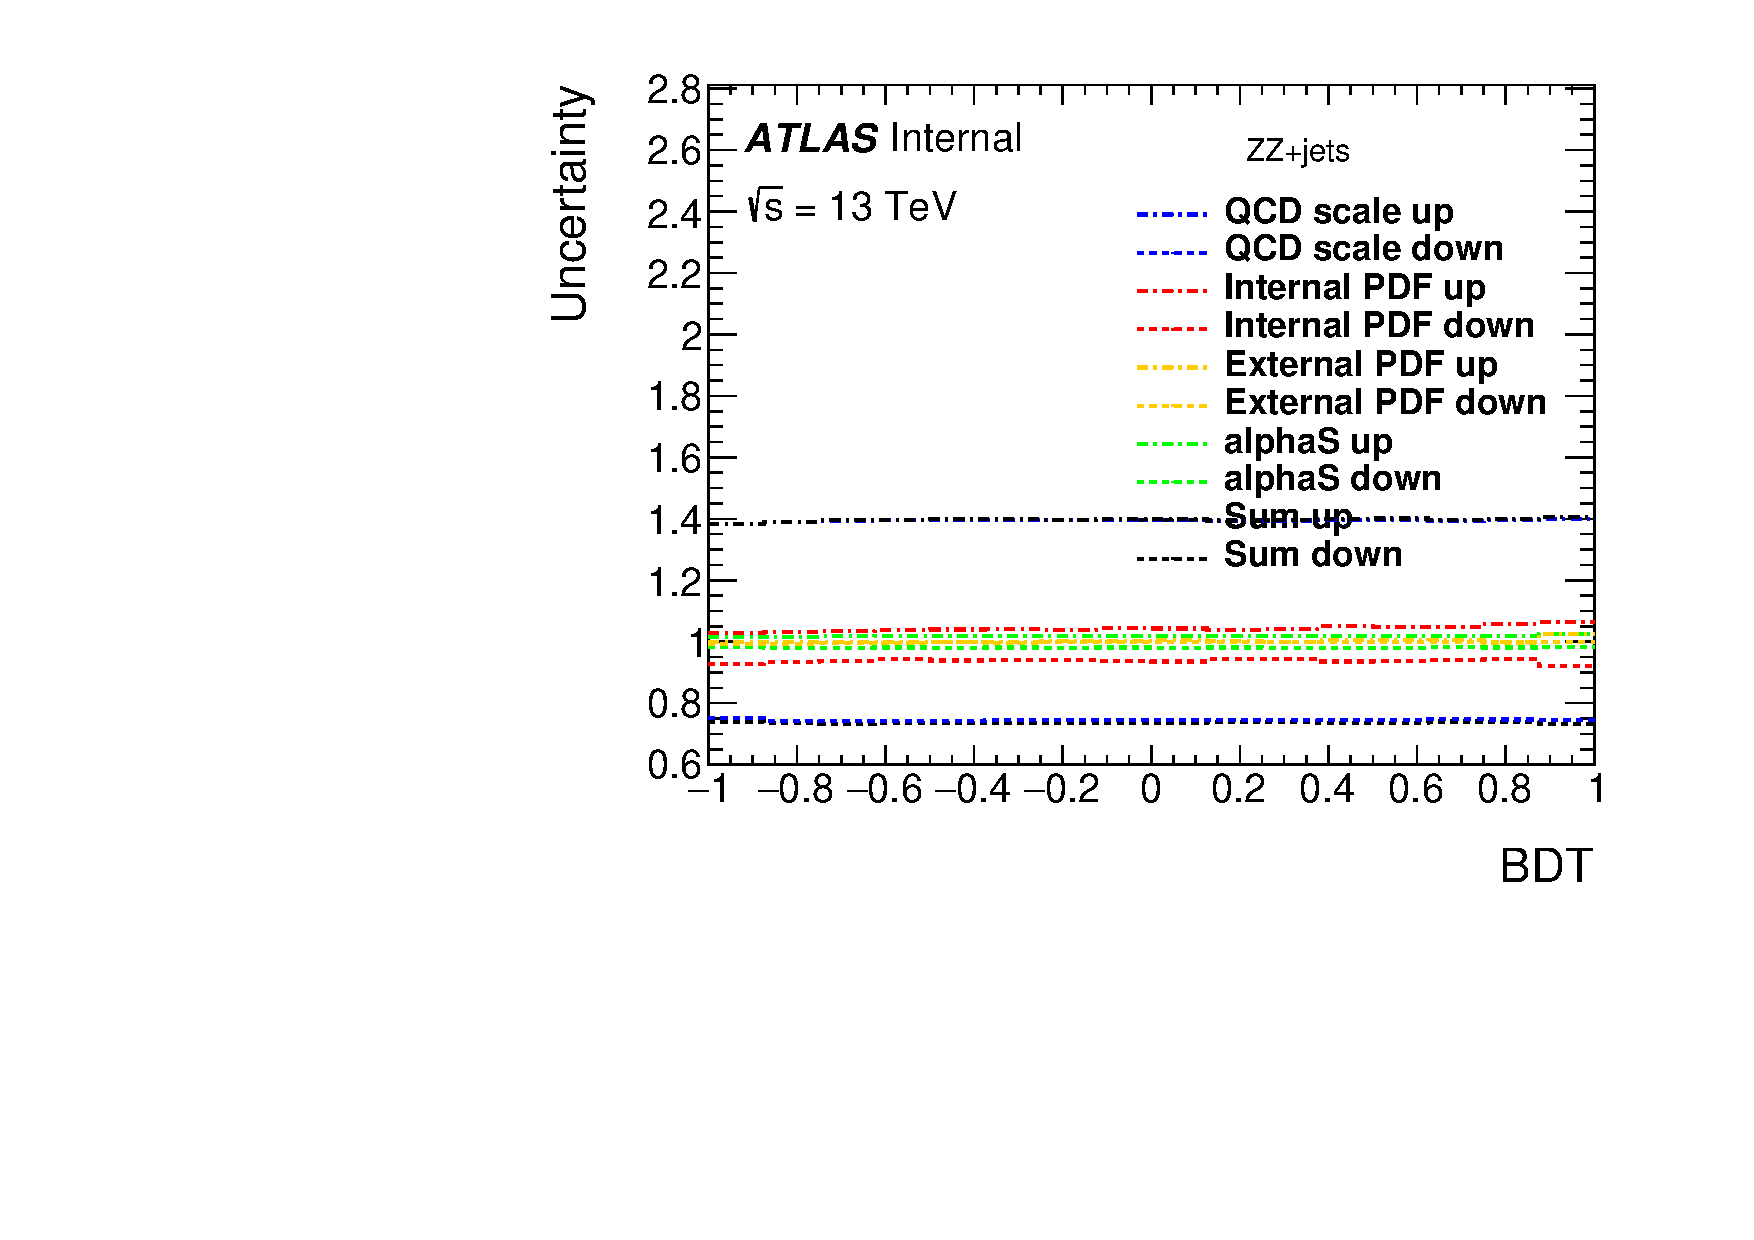
\includegraphics[width=0.48\textwidth]{figures/4l/sys/ggZZ/BDT_SR_linear.pdf}
  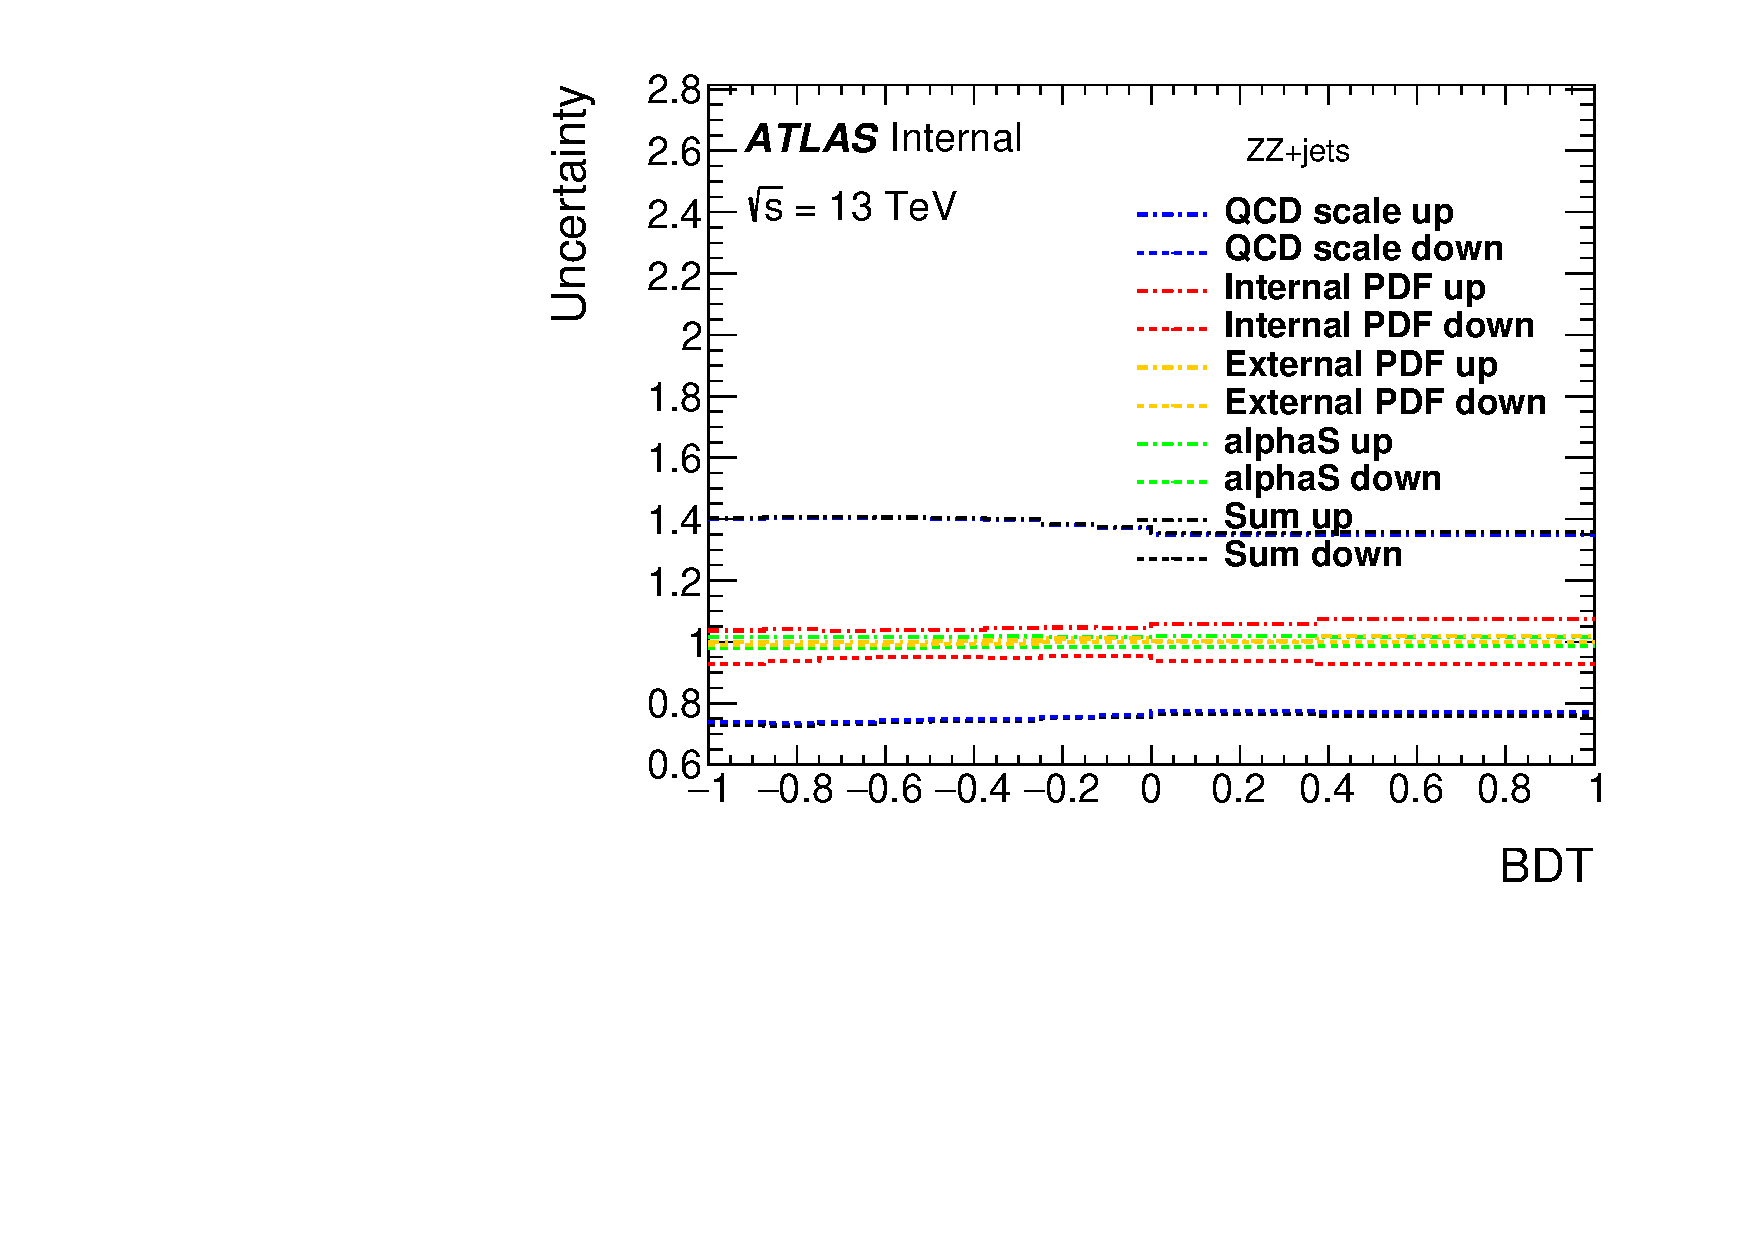
\includegraphics[width=0.48\textwidth]{figures/4l/sys/ggZZ/BDT_CR_linear.pdf}
  \caption{The theoretical uncertainties for \ggZZ background in particle-level SR (left) and CR (right).}
  \label{fig:syst_theo_gg}
\end{figure}


